%=============================================================
% DOCUMENTACIÓN PROYECTO IoT
% Universidad de Talca
%=============================================================
\documentclass[12pt, a4paper]{report}

%-------------------------------------------------------------
% PAQUETES
%-------------------------------------------------------------
\usepackage[utf8]{inputenc}
\usepackage[T1]{fontenc}
\usepackage[spanish]{babel}
\usepackage{graphicx}
\usepackage{geometry}
\usepackage{fancyhdr}
\usepackage{hyperref}
\usepackage{listings}
\usepackage{booktabs}
\usepackage{float}
\usepackage{amsmath}
\usepackage{caption}
\usepackage{subcaption}
\usepackage{enumitem}
\usepackage{setspace}
\usepackage{parskip}

%-------------------------------------------------------------
% DEFINICIÓN LENGUAJE JSON (sin colores)
%-------------------------------------------------------------
\lstdefinelanguage{json}{
  basicstyle=\ttfamily\small,
  morestring=[b]",
  morecomment=[l]{//},
  morecomment=[s]{/*}{*/},
  morekeywords={true, false, null},
  sensitive=false
}

%-------------------------------------------------------------
% GEOMETRÍA DE PÁGINA
%-------------------------------------------------------------
\geometry{
  top=2.5cm,
  bottom=2.5cm,
  left=3cm,
  right=2.5cm
}

%-------------------------------------------------------------
% HIPERVÍNCULOS (sin color)
%-------------------------------------------------------------
\hypersetup{
  colorlinks=false,
  hidelinks,
  pdftitle={Documentación Proyecto IoT},
  pdfsubject={Proyecto IoT}
}

%-------------------------------------------------------------
% ENCABEZADO Y PIE DE PÁGINA
%-------------------------------------------------------------
\pagestyle{fancy}
\fancyhf{}
\fancyhead[L]{\small\textit{Proyecto IoT -- Universidad de Talca}}
\fancyhead[R]{\small
\includegraphics[height=0.6cm]{logoU.png}}
\fancyfoot[C]{\thepage}
\renewcommand{\headrulewidth}{0.4pt}
\renewcommand{\footrulewidth}{0pt}

%-------------------------------------------------------------
% ESTILO DE CÓDIGO (global, sin lenguaje por defecto)
%-------------------------------------------------------------
\lstset{
  basicstyle=\ttfamily\small,
  breaklines=true,
  captionpos=b,
  frame=single,
  numbers=left,
  numberstyle=\tiny,
  showstringspaces=false,
  tabsize=2
}

%-------------------------------------------------------------
% INTERLINEADO
%-------------------------------------------------------------
\setstretch{1.15}

%=============================================================
% INICIO DEL DOCUMENTO
%=============================================================
\begin{document}

%-------------------------------------------------------------
% PORTADA
%-------------------------------------------------------------
\begin{titlepage}
  \centering
  \vspace*{1cm}

  
\includegraphics[width=0.35\textwidth]{logoU.png}\\[1.5cm]

  {\Large \textbf{Universidad de Talca}\\[0.3cm]
   \large Facultad de Ingeniería\\[0.1cm]
   \large Ingeniería Civil en Computación}\\[2cm]

  \rule{\linewidth}{0.5mm}\\[0.4cm]
  {\huge \bfseries Proyecto Casa Clever}\\[0.2cm]
  {\large \textit{Unidad 1 -- 2026}}\\[0.1cm]
  \rule{\linewidth}{0.5mm}\\[2cm]

  \begin{minipage}{0.45\textwidth}
    \begin{flushleft}
      \textbf{Autores:}\\
      Catalina Miño\\
      David Ochoa\\
      Gustavo Torres
    \end{flushleft}
  \end{minipage}
  \begin{minipage}{0.45\textwidth}
    \begin{flushright}
      \textbf{Profesor:}\\
      Ricardo Pérez\\[1cm]
      \textbf{Fecha:}\\
      \today
    \end{flushright}
  \end{minipage}

  \vfill
  {\small Curicó, Chile -- 2026}
\end{titlepage}

%-------------------------------------------------------------
% TABLA DE CONTENIDOS
%-------------------------------------------------------------
\tableofcontents
\newpage

%=============================================================
% SECCIÓN 2: INTRODUCCIÓN Y DESCRIPCIÓN DEL PROBLEMA
%=============================================================
\chapter*{2. Introducción y descripción del problema}
\addcontentsline{toc}{chapter}{2. Introducción y descripción del problema}

La automatización del hogar constituye una de las aplicaciones más extendidas del Internet de las Cosas (IoT). Sistemas capaces de controlar la iluminación, detectar presencia, monitorear la calidad del aire o emitir alertas ante eventos anómalos forman parte ya de soluciones comerciales ampliamente adoptadas, como Google Home, Amazon Alexa o Apple HomeKit.

En este contexto, una familia desea automatizar su hogar con el fin de mejorar la seguridad, el confort y el ahorro energético. Para ello, se requiere un sistema IoT que permita:

\begin{itemize}
  \item Monitorear las condiciones ambientales del hogar (temperatura, humedad y calidad del aire).
  \item Capturar imágenes para identificar si hay una persona presente y quién es.
  \item Recibir alertas automáticas ante rostros desconocidos.
  \item Controlar actuadores de forma automática y manual.
  \item Visualizar toda la información desde un dashboard centralizado accesible en la red local.
\end{itemize}

El presente informe documenta el diseño e implementación de un prototipo funcional que da respuesta a este problema, integrando sensores físicos, comunicación mediante el protocolo MQTT, visión artificial en Node-RED y control automático basado en reglas.

%=============================================================
% SECCIÓN 3: OBJETIVOS
%=============================================================
\chapter*{3. Objetivo general y objetivos específicos}
\addcontentsline{toc}{chapter}{3. Objetivo general y objetivos específicos}

\section*{Objetivo general}

Diseñar e implementar un prototipo IoT funcional que simule la automatización de una vivienda, integrando sensores físicos, comunicación mediante MQTT, visión artificial básica en Node-RED y control automático basado en reglas.

\section*{Objetivos específicos}

\begin{enumerate}
  \item Conectar y programar los sensores del kit asignado en un ESP32.
  \item Utilizar la ESP32-CAM para capturar imágenes y delegar la detección e identificación de personas a un microservicio externo en Python mediante API REST.
  \item Publicar los datos medidos al broker MQTT utilizando una jerarquía de tópicos ordenada.
  \item Diseñar un dashboard en Node-RED que visualice todas las variables del sistema en tiempo real.
  \item Implementar al menos dos estrategias de control automático basadas en umbrales o detección de eventos.
  \item Integrar al menos una notificación externa (Telegram o correo electrónico) ante eventos críticos.
  \item Registrar históricamente los datos en un archivo CSV o base de datos desde Node-RED.
  \item Documentar la arquitectura, decisiones técnicas y resultados en este informe técnico.
\end{enumerate}

%=============================================================
% SECCIÓN 4: ARQUITECTURA DE SOFTWARE Y COMUNICACIÓN
%=============================================================
\chapter*{4. Arquitectura del sistema y comunicación}
\addcontentsline{toc}{chapter}{4. Arquitectura del sistema y comunicación}

La arquitectura de software del proyecto Casa Clever se basa en un ecosistema modular desplegado a través de contenedores utilizando \textbf{Docker Compose}. Esto garantiza que el sistema sea portátil, escalable y fácil de mantener en cualquier red local. El sistema se compone de tres contenedores principales interconectados mediante una red virtual interna (\texttt{iot\_net}):

\begin{itemize}
  \item \textbf{Broker MQTT (Mosquitto):} Actúa como el intermediario de mensajería principal. Se encarga de recibir, encolar y distribuir todos los datos de telemetría de los sensores físicos de forma eficiente.
  \item \textbf{Servidor de Aplicación (Node-RED):} Funciona como el cerebro orquestador y la interfaz gráfica. Contiene el Dashboard accesible por los usuarios, gestiona las reglas lógicas (como el control de actuadores cuando se superan umbrales) y maneja la integración de los servicios.
  \item \textbf{Microservicio de Visión (Python/Flask):} Un contenedor completamente independiente desarrollado en Python. Este servicio expone una API REST encargada de recibir imágenes y utilizar la librería \texttt{face\_recognition} para identificar rostros contra una base de datos local de \textit{caras conocidas}.
\end{itemize}

\section*{Protocolos de comunicación híbridos}

Para optimizar el rendimiento de la red, el sistema separa el tráfico según su naturaleza:
\begin{enumerate}
    \item \textbf{Vía MQTT:} Utilizado por el nodo ESP32 principal para publicar las lecturas de los sensores (temperatura, humedad, niveles de gas y ruido) debido al bajo peso del payload y su fiabilidad.
    \item \textbf{Vía HTTP POST:} Utilizado por el módulo ESP32-CAM. Dado que las imágenes (JPEG) constituyen datos binarios pesados que podrían saturar el broker MQTT, la cámara envía las capturas directamente al servidor mediante peticiones HTTP POST, delegando el análisis biométrico a la arquitectura de contenedores.
\end{enumerate}

\section*{Diagramas de conexiones}

\begin{figure}[H]
    \centering
    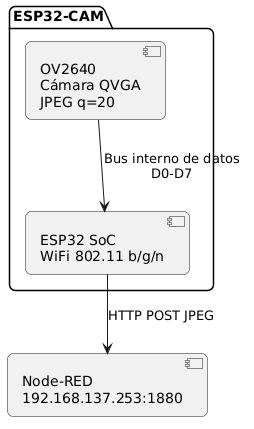
\includegraphics[width=0.3\textwidth]{diagramaCAM.png}
    \caption{Diagrama de conexiones ESP32-CAM}
    \label{fig:diagcam}
\end{figure}

\begin{figure}[H]
    \centering
    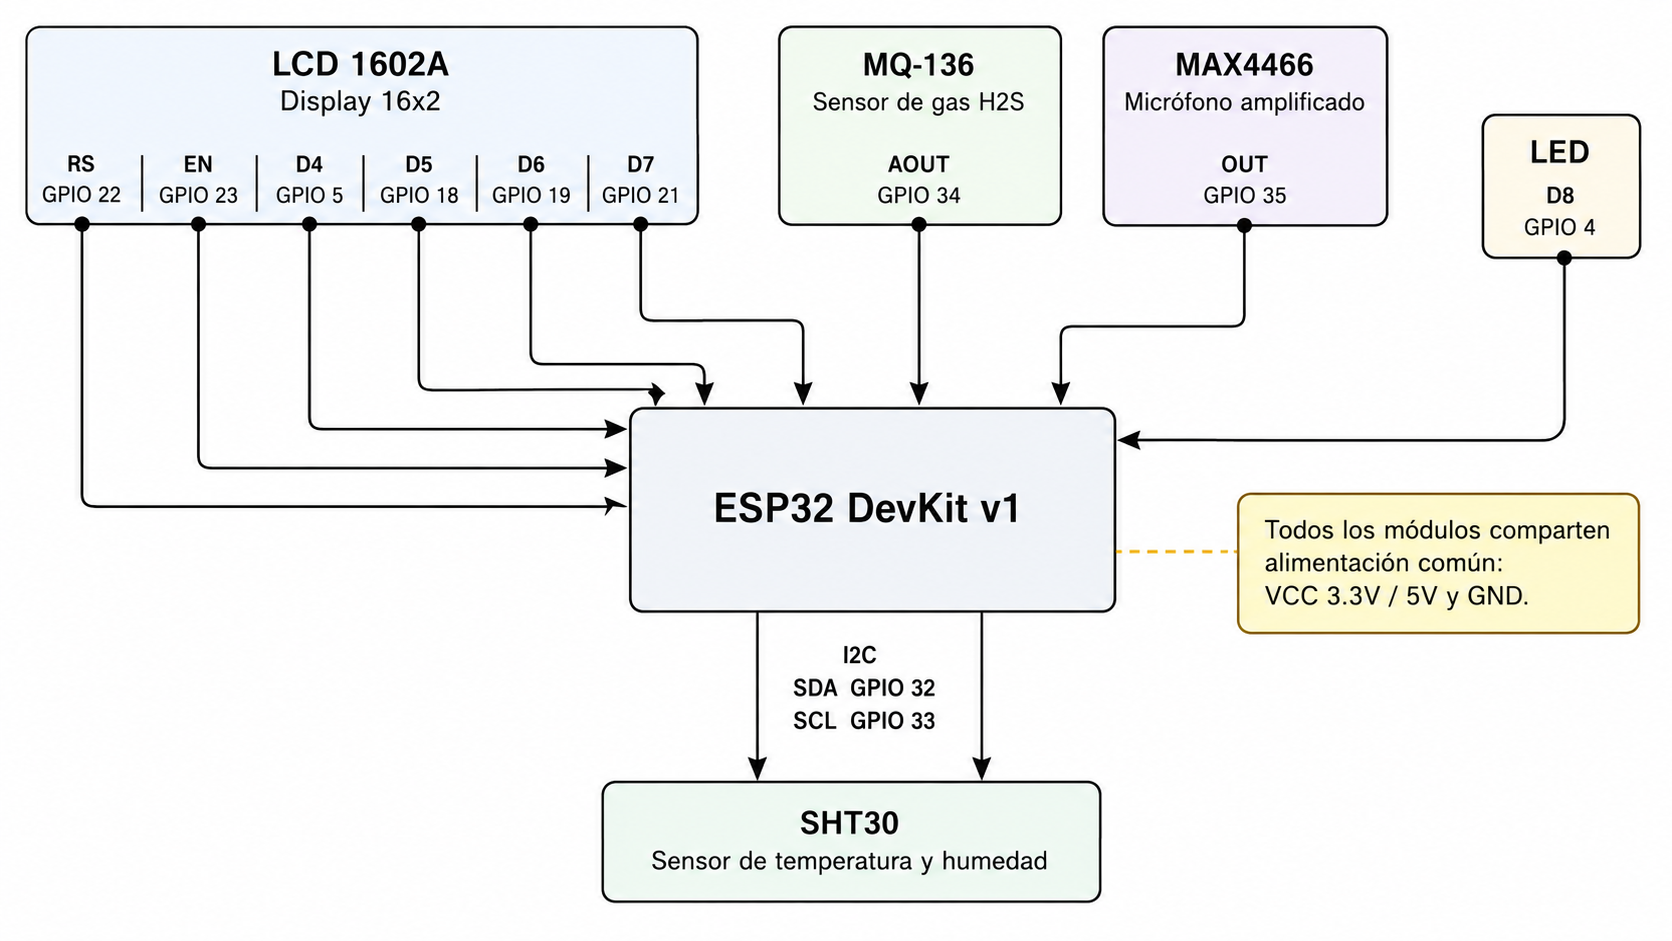
\includegraphics[width=0.9\textwidth]{img nueva.png}
    \caption{Diagrama de conexiones ESP32 (vista esquemática)}
    \label{fig:diagesp32}
\end{figure}

\begin{figure}[H]
    \centering
    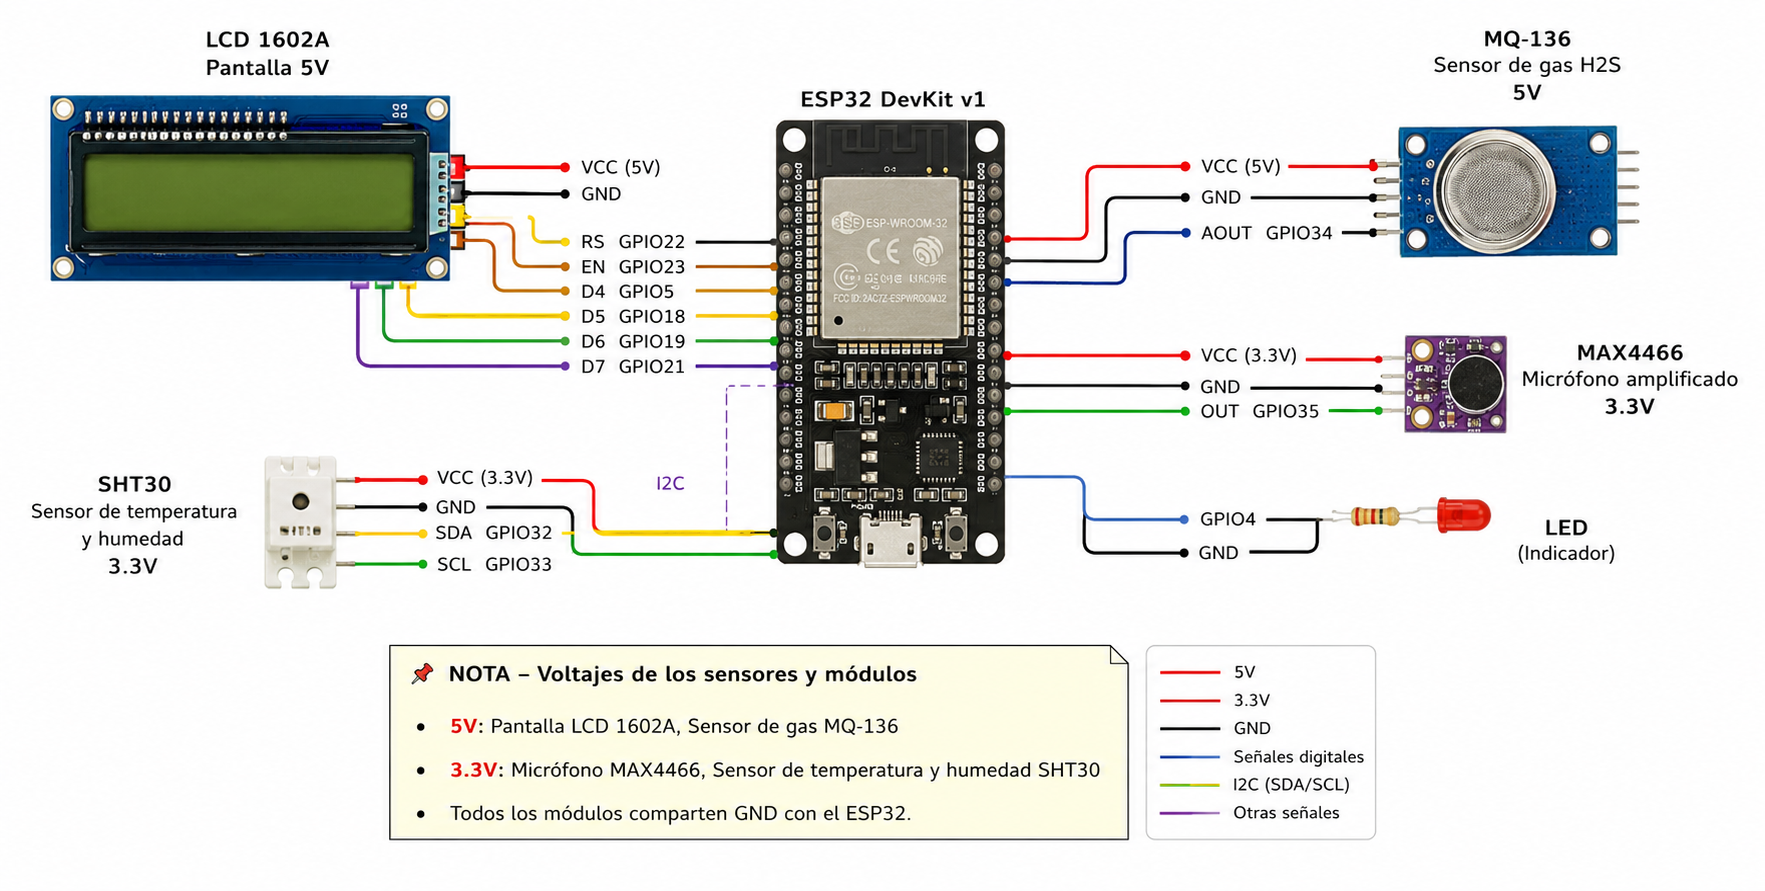
\includegraphics[width=0.9\textwidth]{circuit.png}
    \caption{Diagrama de circuito completo del ESP32}
    \label{fig:circuit}
\end{figure}

%=============================================================
% SECCIÓN 5: DESCRIPCIÓN DE SENSORES
%=============================================================
\chapter*{5. Descripción de cada sensor utilizado y su rol en el sistema}
\addcontentsline{toc}{chapter}{5. Descripción de cada sensor utilizado y su rol en el sistema}

\section*{ESP32 (Microcontrolador principal)}

El ESP32 es un microcontrolador de doble núcleo Xtensa LX6 a 240 MHz, con conectividad Wi-Fi 802.11 b/g/n y Bluetooth 4.2. Actúa como nodo central del sistema: lee los sensores conectados, procesa los datos y los publica al broker MQTT a través de la red local. Su capacidad de conexión inalámbrica lo hace idóneo para aplicaciones IoT domésticas.

\section*{ESP32-CAM (Módulo de cámara)}

El módulo ESP32-CAM combina un microcontrolador ESP32-S con una cámara OV2640 de 2 megapíxeles. En este sistema cumple la función de nodo de visión: captura imágenes del entorno y las transmite a través de peticiones HTTP POST hacia el servidor central. El procesamiento biométrico no ocurre en el módulo ni en Node-RED de forma nativa, sino que es procesado por un contenedor Docker dedicado que corre un microservicio en Python para el reconocimiento facial. Ante la detección de una persona, el sistema genera alertas correspondientes hacia el dashboard y publica la información necesaria.

\section*{Display LCD 1602A (Pantalla local)}

El display 1602A es una pantalla de cristal líquido de 16 columnas y 2 filas, controlada mediante el protocolo I2C a través de un módulo adaptador PCF8574. Su rol en el sistema es mostrar localmente las lecturas más relevantes en tiempo real (temperatura, humedad y estado de alerta), permitiendo consultar el estado del sistema sin necesidad de acceder al dashboard.

\section*{Sensor MQ-136 (Gas -- Sulfuro de hidrógeno)}

El MQ-136 es un sensor electroquímico sensible principalmente al sulfuro de hidrógeno ($H_2S$), aunque también responde a otros gases como $SO_2$ y $NH_3$. Entrega una señal analógica proporcional a la concentración de gas en el ambiente. En el sistema actúa como detector de calidad del aire: cuando el nivel supera un umbral definido, se activa una alerta y se dispara el control automático (buzzer y notificación externa).

\section*{Micrófono MAX4466 (Sensor de nivel sonoro)}

El MAX4466 es un módulo de micrófono con amplificador operacional de ganancia ajustable. Entrega una señal analógica que representa el nivel de presión sonora del entorno. En este proyecto se utiliza como sensor diferencial adicional, detectando eventos sonoros relevantes (golpes, alarmas, voces) que pueden complementar la lógica de detección de presencia.

\section*{Sensor SHT30 (Temperatura y humedad)}

El SHT30 es un sensor digital de temperatura y humedad relativa fabricado por Sensirion, con comunicación I2C. Ofrece precisión de $\pm$0.2°C en temperatura y $\pm$2\% en humedad relativa, con un rango de operación de -40°C a 125°C. Es el sensor ambiental principal del sistema: sus lecturas se publican continuamente al broker MQTT y se visualizan en el dashboard. Además, alimentan las reglas de control automático (por ejemplo, alerta si temperatura $>$ 30°C).



%=============================================================
% SECCIÓN 6: ESTRUCTURA DE TÓPICOS MQTT
%=============================================================
\chapter*{6. Estructura de tópicos MQTT con ejemplos de mensajes JSON}
\addcontentsline{toc}{chapter}{6. Estructura de tópicos MQTT con ejemplos de mensajes JSON}

\section*{Jerarquía de tópicos}

Todos los mensajes se publican bajo el prefijo \texttt{smarthome/equipoXX/}, donde \texttt{equipoXX} identifica al equipo. La siguiente tabla describe cada tópico y su propósito:

\begin{table}[H]
  \centering
  \caption{Jerarquía de tópicos MQTT del sistema}
  \begin{tabular}{p{5.5cm} p{8cm}}
    \toprule
    \textbf{Tópico} & \textbf{Descripción} \\
    \midrule
    \texttt{smarthome/equipoXX/sensores} & Payload JSON agrupado (temperatura, humedad, gas, micrófono) \\[4pt]
    \texttt{smarthome/equipoXX/cámara}   & Detección de rostro \\
    \bottomrule
  \end{tabular}
  \label{tab:topicos}
\end{table}

\section*{Formato de mensajes JSON}

Los mensajes se envían en formato JSON. A continuación se muestra el esquema del mensaje principal publicado por el ESP32 en el tópico \texttt{sensores}:

\begin{lstlisting}[language=json, caption={Mensaje JSON publicado por el nodo de sensores}]
{
    "equipo": "equipoXX",
    "temperatura": 22.12,
    "humedad": 47.93,
    "gas": 1154,
    "microfono": 450
}
\end{lstlisting}

Por otro lado, el microservicio de reconocimiento en Python devuelve su respuesta hacia Node-RED, generando el siguiente formato JSON según el rostro capturado:

\begin{lstlisting}[language=json, caption={Mensaje JSON generado como salida de Python}]
{
    "resultado": "desconocido" 
}
\end{lstlisting}

\textit{Nota: El campo resultado puede tomar valores como "desconocido", "no\_hay\_rostro\_visible" o el nombre de la persona autorizada.}

Los comandos de control enviados desde el dashboard hacia los actuadores siguen el esquema:

\begin{lstlisting}[language=json, caption={Mensaje JSON de comando a actuador}]
{
    "estado": "on"
}
\end{lstlisting}


%=============================================================
% SECCIÓN 7: DASHBOARD
%=============================================================
\chapter*{7. Descripción del dashboard y capturas de pantalla}
\addcontentsline{toc}{chapter}{7. Descripción del dashboard y capturas de pantalla}

El dashboard del sistema Casa Clever fue implementado en \textbf{Node-RED} utilizando el módulo \texttt{@flowfuse/node-red-dashboard} (v1.30.2). Es accesible desde cualquier dispositivo en la red local mediante la dirección \texttt{http://\textless{}IP\_servidor\textgreater{}:1880/dashboard}.

\section*{Componentes del dashboard}

El panel se organiza en una única página principal con cuadrícula adaptable. Sus elementos son:

\begin{itemize}
    \item \textbf{Gauges (medidores de aguja semicircular):} Cuatro indicadores en tiempo real:
    \begin{itemize}
        \item Temperatura: rango 0--50 °C (fuente: \texttt{smarthome/equipoXX/sensores})
        \item Humedad relativa: rango 0--100\% (fuente: \texttt{smarthome/equipoXX/sensores})
        \item Gas (MQ-136): rango 0--495 (fuente: \texttt{smarthome/equipoXX/sensores})
        \item Micrófono (MAX4466): rango variable según nivel sonoro ambiente (fuente: \texttt{smarthome/equipoXX/sensores})
    \end{itemize}
    \item \textbf{Gráficos temporales:} Cuatro gráficos de línea con ventana histórica de \textbf{10 minutos} (interpolación lineal) para temperatura, humedad, gas y micrófono.
    \item \textbf{Estado del reconocimiento facial:} Panel que muestra el último resultado devuelto por el microservicio de visión: nombre del residente autorizado, \texttt{desconocido} o \texttt{no\_hay\_rostro\_visible}.
    \item \textbf{Alertas visuales:} Indicadores activados por los nodos de control cuando se superan umbrales ambientales o se detecta un intruso.
\end{itemize}

\section*{Capturas de pantalla}

\begin{figure}[H]
    \centering
    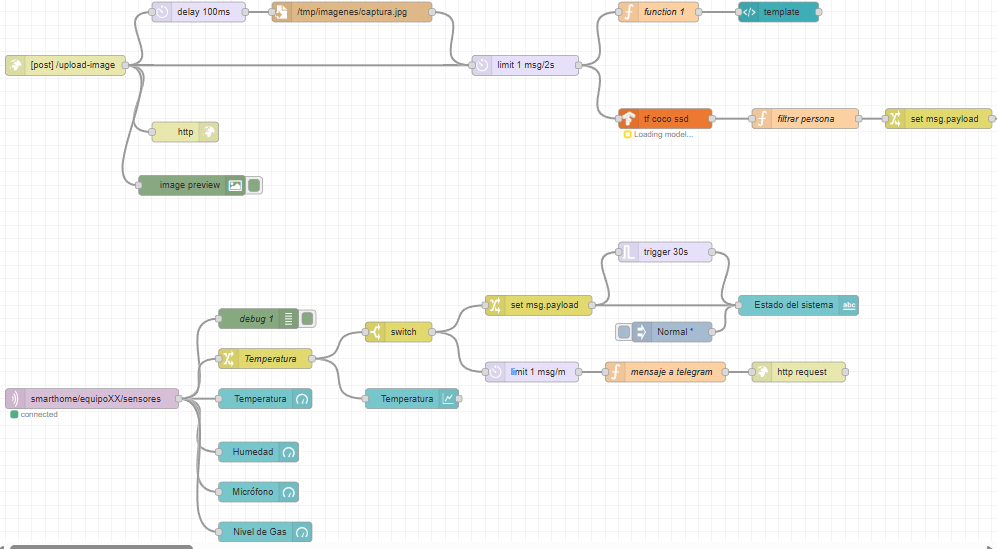
\includegraphics[width=\textwidth]{dashboard.png}
    \caption{Vista general del dashboard en Node-RED con gauges y gráficos temporales}
    \label{fig:dashboard}
\end{figure}

%=============================================================
% SECCIÓN 8: ESTRATEGIAS DE CONTROL
%=============================================================
\chapter*{8. Estrategias de control implementadas}
\addcontentsline{toc}{chapter}{8. Estrategias de control implementadas}

Se implementaron dos estrategias de control automático:

\section*{Control de acceso por reconocimiento facial}

El módulo ESP32-CAM captura una imagen cada 1{,}2 segundos y la envía mediante HTTP POST al servidor Node-RED, que la delega al microservicio Python. El flujo de control es:

\begin{enumerate}
    \item La imagen es analizada por la API de reconocimiento (\texttt{/analizar}) con tolerancia de 0{,}6.
    \item Si el resultado es un nombre autorizado (distinto de \texttt{desconocido} y \texttt{no\_hay\_rostro\_visible}), Node-RED publica el nombre al tópico \texttt{smarthome/equipoXX/camara}.
    \item El ESP32 suscrito activa el actuador de cerradura durante \textbf{4 segundos} (pulso HIGH en GPIO 4).
    \item El nombre reconocido se despliega en el LCD 1602A para confirmación visual local.
    \item Si el rostro es desconocido, se genera una alerta en el dashboard y se activa la notificación externa.
\end{enumerate}

\section*{Control por umbrales ambientales}

Las lecturas de temperatura y humedad son evaluadas en Node-RED mediante nodos \texttt{switch}:

\begin{itemize}
    \item \textbf{Temperatura:} Si supera los 30 °C, se activa una alerta visual en el dashboard y se envía notificación por Telegram.
    \item \textbf{Humedad relativa:} Si cae por debajo del umbral mínimo definido, se genera una alerta en el dashboard y se envía la notificación correspondiente.
\end{itemize}

%=============================================================
% SECCIÓN 9: NOTIFICACIONES Y REGISTRO HISTÓRICO
%=============================================================
\chapter*{9. Notificaciones}
\addcontentsline{toc}{chapter}{9. Notificaciones}

\section*{Notificaciones externas (Telegram)}

El sistema envía notificaciones automáticas mediante un bot de \textbf{Telegram}, integrado en Node-RED a través de nodos HTTP Request hacia la API de Telegram. Las notificaciones se activan ante los siguientes eventos:

\begin{itemize}
    \item \textbf{Temperatura} ambiental superior al umbral definido (30 °C).
    \item \textbf{Humedad relativa} fuera del rango aceptable.
\end{itemize}

Cada mensaje incluye el tipo de evento, el valor medido y la marca de tiempo.

%=============================================================
% SECCIÓN 10: PROBLEMAS Y SOLUCIONES
%=============================================================
\chapter*{10. Problemas encontrados y soluciones aplicadas}
\addcontentsline{toc}{chapter}{10. Problemas encontrados y soluciones aplicadas}

\section*{Latencia en la transmisión de imágenes (ESP32-CAM)}

\textbf{Problema:} El módulo ESP32-CAM transmite las imágenes capturadas hacia Node-RED mediante HTTP POST. Durante las pruebas se observó una latencia significativa: las imágenes llegaban al servidor con un retraso notorio respecto al momento de captura, degradando la efectividad del sistema de reconocimiento facial en tiempo real.

\textbf{Análisis:} El protocolo HTTP introduce una sobrecarga considerable al establecer una nueva conexión TCP por cada imagen enviada (\textit{connection overhead}), sumado al tiempo de serialización y transmisión del payload JPEG a través de Wi-Fi. A diferencia de MQTT, que mantiene una conexión persistente y está optimizado para datos pequeños y frecuentes, HTTP no fue diseñado para el streaming continuo de datos binarios.

\textbf{Solución intentada:} No fue posible eliminar la latencia de forma satisfactoria dentro del alcance del proyecto. Como medida de mitigación, se ajustó el intervalo de captura a \textbf{1{,}2 segundos} entre imágenes, buscando un equilibrio entre la cantidad de imágenes procesadas y la carga sobre la red. A pesar de este ajuste, el protocolo HTTP continúa siendo un cuello de botella que impide lograr una transmisión fluida y en tiempo real.

\textbf{Posibles mejoras futuras:} Para resolver este problema de raíz se recomienda migrar a protocolos diseñados para streaming continuo, como \textbf{WebSockets} o \textbf{RTSP} (Real Time Streaming Protocol), que mantienen una conexión persistente y reducen drásticamente la latencia de transmisión imagen a imagen.

%=============================================================
% SECCIÓN 11: CONCLUSIONES
%=============================================================
\chapter*{11. Conclusiones}
\addcontentsline{toc}{chapter}{11. Conclusiones}

El desarrollo del proyecto Casa Clever permitió integrar exitosamente un conjunto de tecnologías IoT en un prototipo funcional de automatización de hogar. Los principales aprendizajes obtenidos son:

\begin{enumerate}
    \item \textbf{Arquitectura modular con Docker:} El uso de contenedores Docker Compose demostró ser una decisión acertada, permitiendo desplegar y mantener el sistema de forma ordenada, con servicios independientes y reemplazables sin afectar al resto del sistema.

    \item \textbf{MQTT como protocolo de telemetría:} El protocolo MQTT resultó altamente eficiente para la transmisión continua de datos de sensores, con baja latencia y consumo mínimo de recursos en el ESP32, validando su elección frente a alternativas como HTTP para este tipo de datos.

    \item \textbf{Reconocimiento facial distribuido:} Delegar el procesamiento de visión artificial a un microservicio Python independiente fue la estrategia correcta, dado que el ESP32-CAM no posee la capacidad computacional para ejecutar modelos de reconocimiento localmente.

    \item \textbf{Limitaciones del protocolo HTTP para imágenes:} La transmisión de imágenes vía HTTP POST introdujo una latencia no eliminable dentro del alcance del proyecto, evidenciando la necesidad de protocolos de streaming (WebSockets, RTSP) para aplicaciones de videovigilancia en tiempo real.

    \item \textbf{Node-RED como orquestador:} Node-RED demostró ser una herramienta poderosa y flexible para integrar múltiples fuentes de datos, aplicar lógica de control basada en reglas y construir dashboards interactivos sin necesidad de desarrollar un backend personalizado.

    \item En términos generales, el proyecto cumplió con los objetivos planteados: monitoreo ambiental en tiempo real, control de acceso basado en reconocimiento facial y notificaciones externas ante eventos críticos de temperatura y humedad.
\end{enumerate}

\end{document}